% $Header: svn+ssh://andre@crapman/home/junda/repos/andre/school/trunk/m/Chapter/stat/probability/chapter/prob.intro.tex 221 2021-02-13 18:18:09Z andre $
\tikzsetfigurename{ch.00.01.intro}
% \tikzexternaldisable
% \tikzexternalenable

% \part{Kombi}
\section{\label{sec0002_intro}Intro}
\subsection*{Naturwissenschaftliche Arbeitsweisen}
%= = = = = = = = = = = = = = = = = = = = = = = = = = = = = = = = = = = = = = =
%= = = = = = = = = = = = = = = = = = = = = = = = = = = = = = = = = = = = = = =
% \iffalse
\begin{frame}
  \frametitle{Naturwissenschaftliche Arbeitsweisen}
  \framesubtitle{Vom Glauben zum Wissen}
  %%= = = = = = = = = = = = = = = = = = = = = = = = = = = = = = = = = = = = = =
  \begin{block}{Wades Spirale}
    \parbox[t]{0.36\linewidth}{
      \begin{tikzpicture}[scale=1,x=1cm,y=1cm
          ,baseline={([yshift=-0.7\baselineskip]current bounding box.north)}
          ,>={Stealth[length=2.5mm,round,open]}
          ,line cap=round,line join=round,inner sep=1pt,outer sep=2pt
        ]
        \path[use as bounding box] (-2,-2) rectangle (2,2);
        \ifteacher
          \only<1-3,5->{\node at (0,0) {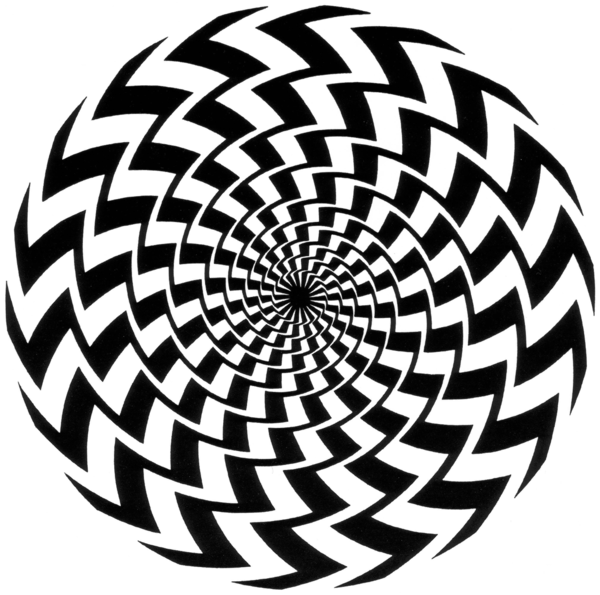
\includegraphics[width=0.93\linewidth]{./chapter/00.intro/pics/wadesSpirale.sm.png}};}
          \foreach \x in {20,16,12,9,4}{
            \only<3->{\draw[red,thick] (0,0) circle(\x mm);}
          }
        \else
          {\node at (0,0) {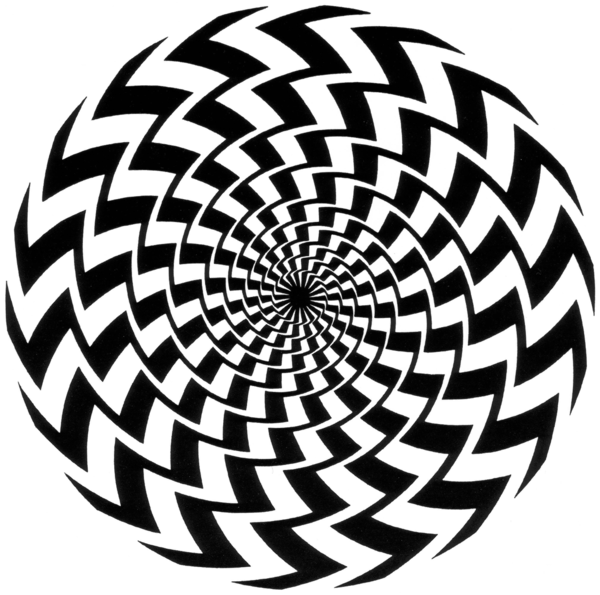
\includegraphics[width=0.93\linewidth]{./chapter/00.intro/pics/wadesSpirale.sm.png}};}
          % \foreach \x in {20,16,12,9,4}{
          %   {\draw[red,thick] (0,0) circle(\x mm);}
          % }
        \fi
      \end{tikzpicture}\\
      {\tiny from \cite[\tiny Apolin 2017, Big Bang 5 RG: \emph{1.1 Im Falle eines Falles}]{apolin2017:bigBang5RG}}
    }\hspace{\stretch{1}}\parbox[t]{0.62\linewidth}{
      \begin{itemize}
        \item <2-> Ist das eine Spirale? 
        \item <3-> \ifteacher Oder doch nur Kreise?
                   \else Zeichnen Sie Kreise ein.
                   \fi
        \item <5-> Die Behauptung (\ifteacher{}Hypothese\else \fbox{\phantom{Hypothese}}\fi),
          dass es eine \ifteacher Spirale \else \fbox{\phantom{Spirale}}\fi
          sei,  konnte widerlegt (\ifteacher{}falsifiziert\else \fbox{\phantom{falsifiziert}}\fi)
          werden.
      \end{itemize}
      \only<6->{\ifteacher In der Naturwissenschaftlichen Arbeitsweise werden
        \emph{Hypothesen} aufgestellt, die durch Experimente
        \emph{widerlegt} (falsifiziert) werden können.
        \else\fi}
    }
  \end{block}
  %%= = = = = = = = = = = = = = = = = = = = = = = = = = = = = = = = = = = = = =
\end{frame}
%==============================================================================

% \section{Intro}
% \subsection*{Naturwissenschaftliche Arbeitsweisen}
%= = = = = = = = = = = = = = = = = = = = = = = = = = = = = = = = = = = = = = =
%= = = = = = = = = = = = = = = = = = = = = = = = = = = = = = = = = = = = = = =
% \iffalse
\begin{frame}
  \frametitle{Naturwissenschaftliche Arbeitsweisen}
  \framesubtitle{Vom Fallen}
  %%= = = = = = = = = = = = = = = = = = = = = = = = = = = = = = = = = = = = = =
  \parbox[t]{0.2\linewidth}{\raisebox{\dimexpr-0.8\height+\ht\strutbox}{%%
    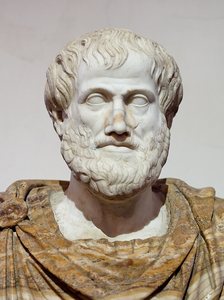
\includegraphics[width=0.99\linewidth]{./chapter/00.intro/pics/800px-Aristotle_Altemps_Inv8575.sm.png}}}
  \hspace{\stretch{1}}\parbox[t]{0.79\linewidth}{
    Lange Zeit glaubte man, dass schwere K\"orper schneller fallen als leichte
    (Aristoteles).
    Wie kann das \ifteacher{}widerlegt\else\fbox{\phantom{widerlegt}}\fi{}
    oder \ifteacher{}best\"atigt\else\fbox{\phantom{best\"atigt}}\fi{} werden?
    \\\vspace{\stretch{1}}
    {\tiny \cite[\url{https://upload.wikimedia.org/wikipedia/commons/a/ae/Aristotle_Altemps_Inv8575.jpg}]{enwiki:main}}
  }\\
  \pause
  \visible<+->{
    \begin{block}{Reales Experiment}
      \begin{itemize}
        \item<+-> Zwei Steine mit unterschiedlicher Masse werden
          \ifteacher{}gleichzeitig\else\fbox{\phantom{gleichzeitig}}\fi{}
          aus der \ifteacher{}gleichen\else\fbox{\phantom{gleichen}}\fi{}
          H\"ohe fallen gelassen.
        \item<+-> Durch \adSTField[1]{Beobachtung} beziehungsweise auch 
          \adSTField[2]{Messung} wird festgestellt, dass beide Steine
          \adSTField[2]{gleichenschnell} auf dem Boden aufkommen.
      \end{itemize}
    \end{block}
  }
  %%= = = = = = = = = = = = = = = = = = = = = = = = = = = = = = = = = = = = = =
\end{frame}
%==============================================================================

% \section{Intro}
% \subsection*{Naturwissenschaftliche Arbeitsweisen}
%= = = = = = = = = = = = = = = = = = = = = = = = = = = = = = = = = = = = = = =
%= = = = = = = = = = = = = = = = = = = = = = = = = = = = = = = = = = = = = = =
% \iffalse
\begin{frame}
  \frametitle{Naturwissenschaftliche Arbeitsweisen}
  \framesubtitle{Vom Fallen}
  %%= = = = = = = = = = = = = = = = = = = = = = = = = = = = = = = = = = = = = =
  
  Lange Zeit glaubte man, dass schwere K\"orper schneller fallen als leichte.
  Wie kann das \ifteacher{}widerlegt\else\fbox{\phantom{widerlegt}}\fi{}
  oder \ifteacher{}best\"atigt\else\fbox{\phantom{best\"atigt}}\fi{} werden?
  \pause
  \visible<+->{
    \begin{block}{Gedankenexperiment}
      \parbox[t]{0.3\linewidth}{
        \raisebox{\dimexpr-1.2\height+\ht\strutbox}{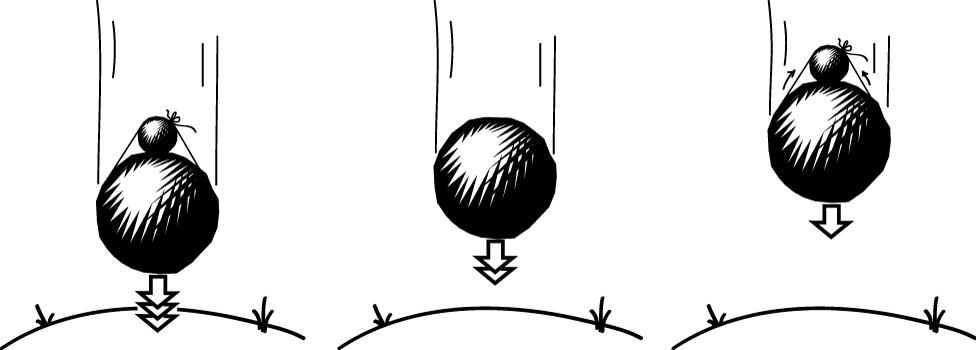
\includegraphics[width=0.98\linewidth]{./chapter/00.intro/pics/fallingStones.png}}\\
        {\tiny \url{https://personal.lse.ac.uk/robert49/ebooks/philsciadventures/img/balls2.gif}}
      }\hspace{\stretch{1}}\parbox[t]{0.69\linewidth}{
       \begin{itemize}
         \item<+-> \textbf{links}: Gro\ss{}er und kleiner Stein zusammen w\"urden
           \ifteacher{}schneller\else\fbox{\phantom{schneller}}\fi{}
           fallen (Aristoteles) als 
         \item<+-> \textbf{mitte}: der gro\ss{}e Stein alleine fallen w\"urde.
         \item <+-> \textbf{rechts}: der kleine Stein f\"allt laut Aristoteles
           \ifteacher{}langsamer\else\fbox{\phantom{langsamer}}\fi{} als der
           gro\ss{}e Stein, und w\"urde daher den gro\ss{}en Stein bremsen.
       \end{itemize}
      }
      \visible<+->{Das f\"uhrt zu einem \adSTField[1]{Widerspruch} zu Aristoteles,
      und veranlasste \adSTField[]{Galileo Galilei} zu der Annahme, dass
      alle K\"orper \adSTField[]{gleichschnell} fallen.}
    \end{block}
  }
  %%= = = = = = = = = = = = = = = = = = = = = = = = = = = = = = = = = = = = = =
\end{frame}
%==============================================================================

% \section{Intro}
% \subsection*{Naturwissenschaftliche Arbeitsweisen}
%= = = = = = = = = = = = = = = = = = = = = = = = = = = = = = = = = = = = = = =
%= = = = = = = = = = = = = = = = = = = = = = = = = = = = = = = = = = = = = = =
% \iffalse
\begin{frame}
  \frametitle{Naturwissenschaftliche Arbeitsweisen}
  \framesubtitle{Das Experiment}
  %%= = = = = = = = = = = = = = = = = = = = = = = = = = = = = = = = = = = = = =
  \parbox[t]{0.3\linewidth}{
    \raisebox{\dimexpr-1\height+\ht\strutbox}{%%
      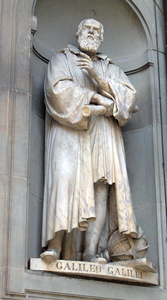
\includegraphics[width=0.75\linewidth]{./chapter/00.intro/pics/Galileo_Galilei01.sm.png}}\\
    {\tiny Von User:JoJan - Eigenes Werk, CC BY-SA 3.0, 
     \url{https://commons.wikimedia.org/w/index.php?curid=408982}
     \url{https://commons.wikimedia.org/wiki/File:Galileo_Galilei_2.jpg}}
  }\hspace{\stretch{1}}\parbox[t]{0.69\linewidth}{
  \adSTField[]{Galileo Galilei} f\"uhrte \adSTField[]{falsifizierbare} 
    Experimente ein, und begr\"undet damit die \adSTField[]{moderne 
    Naturwissenschaft}.
  \pause
  Aus einer \adSTField[2]{Behauptung} (Hypothese) wird ein
  \adSTField[2]{Experiment} abgeleitet, das die Hypothese
  \adSTField[2]{widerlegen} (falsifizieren) kann.\pause{} Wird durch 
  Experimente die Hypothese nicht widerlegt, so ist sie
  \adSTField[2]{best\"atigt}, aber nicht bewiesen, und wird 
  zu einer \adSTField[2]{Theorie} erhoben. 
  \pause 
  Von Galileo Galilei stammt auch der Ausspruch:
  \pause
  \begin{quote}
    {Alles, was messbar ist, messen, \\
    alles was nicht messbar ist, 
    messbar machen.}
  \end{quote}
  \pause 
  Nach \adSTField[1]{Sir Karl Raimund Popper} ist eine Theorie nur dann
  \adSTField[1]{wissenschaftlich}, wenn sie \adSTField[1]{falsifizierbar} ist.
 }
  %%= = = = = = = = = = = = = = = = = = = = = = = = = = = = = = = = = = = = = =
\end{frame}
%==============================================================================

\mode<beamer>{%%
% \section{Intro}
% \subsection*{Naturwissenschaftliche Arbeitsweisen}
%= = = = = = = = = = = = = = = = = = = = = = = = = = = = = = = = = = = = = = =
%= = = = = = = = = = = = = = = = = = = = = = = = = = = = = = = = = = = = = = =
% \iffalse
\begin{frame}
  \frametitle{Naturwissenschaftliche Arbeitsweisen}
  \framesubtitle{Reference}
  %%= = = = = = = = = = = = = = = = = = = = = = = = = = = = = = = = = = = = = =
{
\printbibliography[segment=\therefsegment,heading=subbib]
% \printbibliography[segment=\therefsegment,heading=subbibliography,title={Online Sources}]
}
\end{frame}
%==============================================================================
}

% % \section{Intro}
% \subsection*{Intro}
% %= = = = = = = = = = = = = = = = = = = = = = = = = = = = = = = = = = = = = = =
% %= = = = = = = = = = = = = = = = = = = = = = = = = = = = = = = = = = = = = = =
% % \iffalse
% \begin{frame}
%   \frametitle{Modelle}
%   \framesubtitle{Settings}
% %  \framesubtitle{Settings I}
%   %%= = = = = = = = = = = = = = = = = = = = = = = = = = = = = = = = = = = = = =
%
% \begin{block}{Settings I}
%   Die Kugeln werden nach der Ziehung
%   \begin{description}
%     \item [wieder zur\"uckgelegt]: der Ball kann daher \"ofter
%         gezogen werden, oder
%     \item [zur Seite gelegt]: dann wird der Ball maximal
%   einmal gezogen.
%   \end{description}
% \end{block}
%
% \pause
% \begin{block}{Settings II}
%   In der Urne befinden sich Kugeln, die
%   \begin{description}
%     \item [unterscheidbar sind]: jeder Ball ist ein Unikat (Farbe, Nummer,
%         Material, \dots)
%     \item [nicht unterscheidbar sind]: es gibt B\"alle, die die gleichen
%         Eigenschaften haben (z.~B. drei blaue und zwei rote B\"alle)
%   \end{description}
% \end{block}
%
% \end{frame}
% %==============================================================================
%
% % \section{Intro}
% % \subsection*{Modelle}
% %= = = = = = = = = = = = = = = = = = = = = = = = = = = = = = = = = = = = = = =
% %= = = = = = = = = = = = = = = = = = = = = = = = = = = = = = = = = = = = = = =
% % \iffalse
% \begin{frame}
%   \frametitle{Modelle}
%   \framesubtitle{Settings}
%   %%= = = = = = = = = = = = = = = = = = = = = = = = = = = = = = = = = = = = = =
%
% \begin{block}{Settings III}
%   Aus einer Urne mit $n$ Kugeln werden $k$ B\"alle gezogen.
%   \begin{description}
%     \item [$k=n$]: Permutationen
%     \item [$k<n$]: Variationen (alle B\"alle sind unterscheidbar)
%       und Kombinationen (B\"alle mit gleichen Eigenschaften)
%   \end{description}
% \end{block}
%
% \pause
% Aus wikipedia {\tiny(\url{https://de.wikipedia.org/wiki/Abz\%C3\%A4hlende_Kombinatorik\#Begriffsabgrenzungen})}:\\
% % https://de.wikipedia.org/wiki/Abz%C3%A4hlende_Kombinatorik#Begriffsabgrenzungen
% {\tiny
% Aufgrund der Vielfalt der Herangehensweisen sind die Schreibweisen und
% Begrifflichkeiten im Bereich der Kombinatorik leider oft recht uneinheitlich.
% Zwar bezeichnen übereinstimmend alle Autoren die Vertauschung der Reihenfolge
% einer Menge von $n$ unterscheidbaren Elementen als Permutation. W\"ahlt man
% dagegen von diesen $n$ Elementen nur $k < n$  Elemente aus, deren Reihenfolge
% man anschließend vertauscht, bezeichnen viele Autoren das nun als Variation,
% geordnete Stichprobe bzw. Kombination mit Berücksichtigung der Reihenfolge,
% andere dagegen (namentlich im englischsprachigen Raum) weiter als Permutation.
% L\"asst man schließlich in einer solchen Auswahl von Elementen deren
% Reihenfolge au\ss{}er Acht, wird solch eine Auswahl nun für gew\"ohnlich
% ungeordnete Stichprobe, Kombination ohne Berücksichtigung der Reihenfolge
% oder einfach nur Kombination genannt. Kombinationen sind also, sofern
% nichts weiter zu ihnen gesagt wird, in der Regel ungeordnet, Permutationen
% und/oder Variationen dagegen geordnet, wobei die Frage, ob man Permutationen
% als Sonderf\"alle von Variationen (oder umgekehrt) betrachtet, gegebenenfalls
% von Autor zu Autor unterschiedlich beantwortet wird.\\
% Alles in allem gibt es also zunächst einmal drei (oder auch nur zwei)
% verschiedene Fragestellungen, die ihrerseits noch einmal danach unterteilt
% werden, ob es unter den ausgewählten Elementen auch Wiederholungen gleicher
% Elemente geben darf oder nicht. Ist ersteres der Fall, spricht man von
% Kombinationen, Variationen oder Permutationen mit Wiederholung, andernfalls
% solchen ohne Wiederholung. Stellt man sich schließlich vor, dass die
% ausgew\"ahlten Elemente dabei einer Urne oder Ähnlichem entnommen werden,
% wird dementsprechend auch von Stichproben mit oder ohne Zur\"ucklegen
% gesprochen.\\
% }
%
% \end{frame}
% %==============================================================================
